\subsection{MLOps}

The deployment model is based on a two-path parallel strategy that addresses both geographic expansion and partnership integration. The first strategy employs a phased city district roll-out, beginning with a small pilot in 1-2 high-demand areas with 100-200 sensor-equipped vehicles. This initial roll-out demonstrates the core value proposition while maintaining low infrastructure complexity. After positive validation, the expansion phase extends coverage to 5-10 additional districts, scaling to 1,000-2,000 vehicles and implementing the first model updates derived from real-world data. Concurrently, a partnership-led deployment strategy targets existing fleets—taxi, delivery fleets, car-sharing etc—to maximize coverage thanks to vehicles that already travel through dense urban areas.

The MLOps pipeline design employs a multi-stage approach optimized for distributed networks. Data collection begins at the vehicle level, where ultra-low-power proximity sensors detect close-by parking spaces with signals preprocessed by onboard micro controllers to eliminate noise and normalize formats (if possible). This edge computing approach significantly reduces transmission overhead. The data pipeline implements strict data anonymization regarding vehicle identifiers, such that the data sent from the vehicle is limited to location coordinates and timestamps only. Telemetry aggregates are stored in cloud storage by district and timestamp to enable both historical analysis and real-time serving. Automated quality assurance operations check for spatial consistency and detect anomalous patterns that may be indicative of sensor faults or tampering incidents. The training infrastructure utilizes containerized environments with Graph Neural Network (GNN) components specifically optimized for the spatial relationships inherent in parking networks Training runs are based on a double-trigger system—time-scheduled (weekly for pilot, monthly for expansion) and threshold-triggered when measures of performance indicate drift outside of acceptable parameters. The assessment process uses champion-challenger competitions where new models run in shadow mode, making decisions on real data but not influencing actions. Model deployment follows a canary release form, growing incrementally from one district to the entire network, with automatic rollback capability triggered by anomaly detection systems that monitor technical performance, as well as user-reported satisfaction measures. 

Regarding Cloud infrastructure deployment providers, we decided to architect the infrastructure using AWS, but alternatives such as Microsoft Azure are also viable. The AWS system relies on EC2 Spot Instances for cost-effective training, alongside reserved instances for stable inference, with data flowing through a data lake in S3 with partitioned buckets (raw, processed, models) and real-time availability served by DynamoDB. Containerized microservices executed by ECS/Fargate manage the model life cycle from training to evaluation and phased deployment, while SageMaker components offer version control, automated workflow, explainability and drift detection. Azure also facilitates these through AKS, IoT Hub, Blob Storage, Cosmos DB and Azure ML, albeit with enterprise benefits for city-level deployments.
\begin{figure}[H]
    \centering
    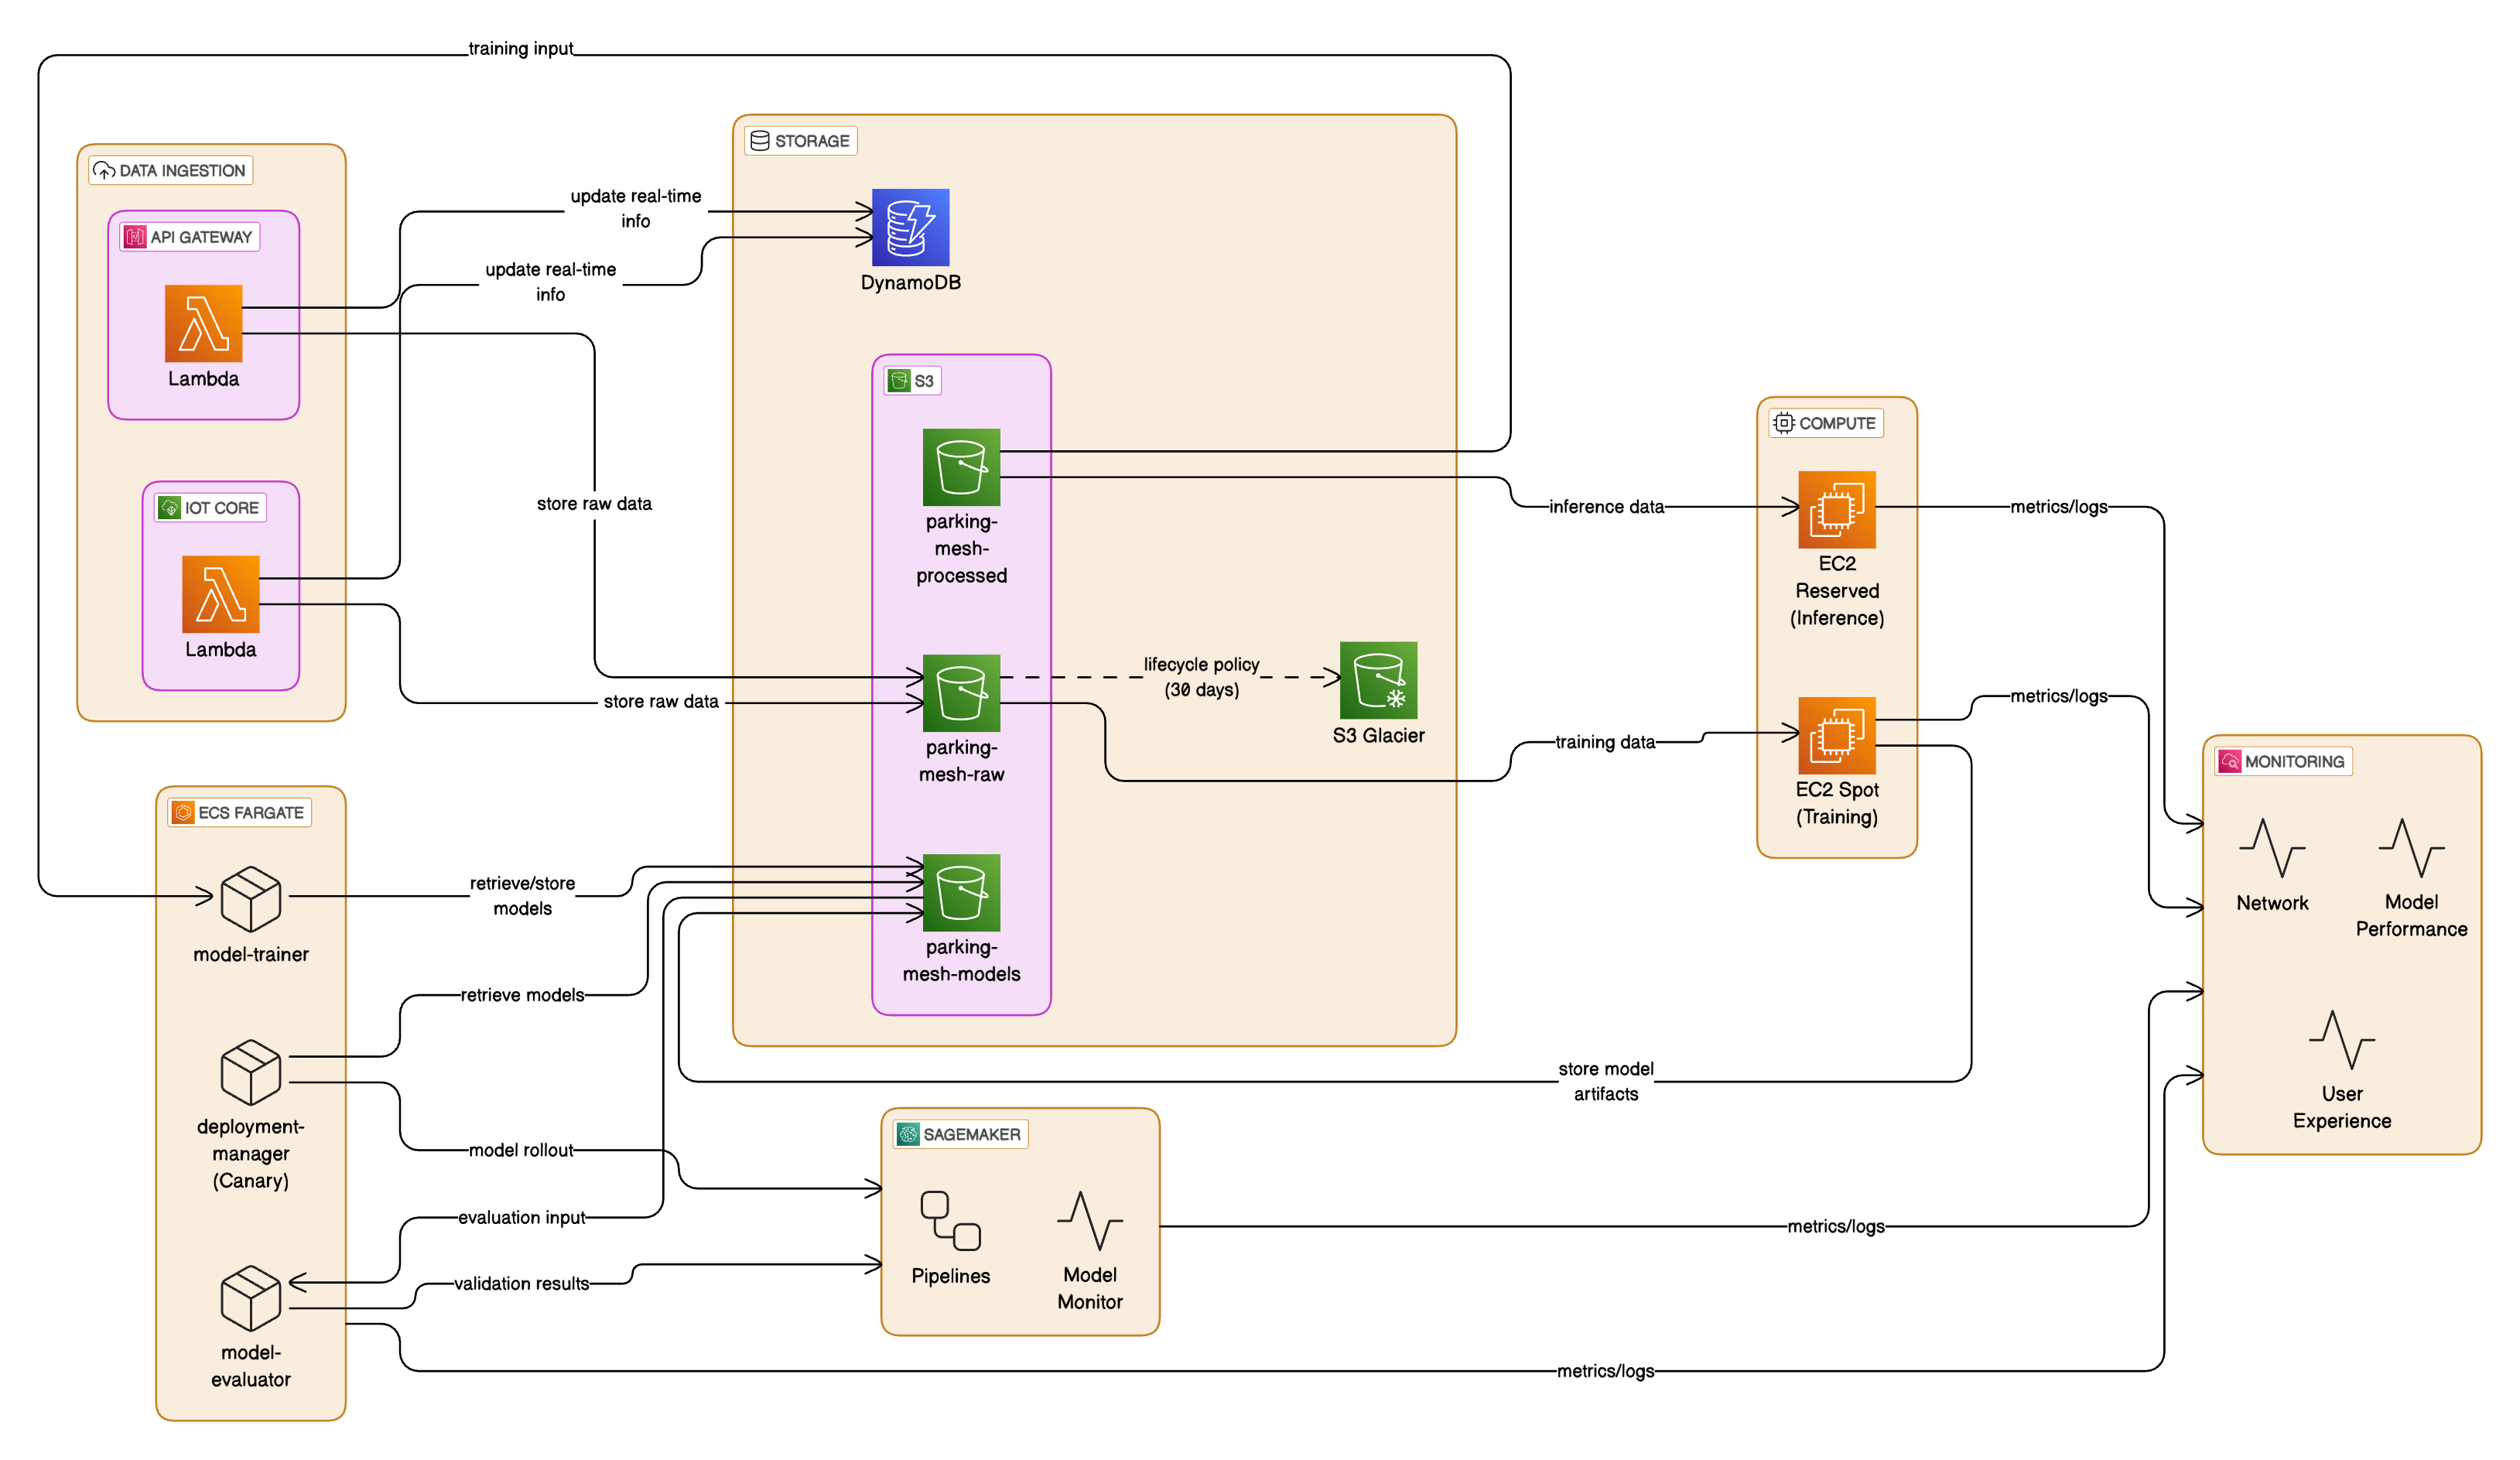
\includegraphics[width=\linewidth]{Figures/mlops.png} % increased from 0.8 to 1.0
    \captionsetup{justification=centering}
    \caption{Diagram of cloud infrastructure.}
    \label{fig:Deployment}
\end{figure}